\documentclass[12pt]{article}

\usepackage{notestyle}

\graphicspath{{./img/}}


\title{Notes Optimization}
\author{Brendon Mendicino}


\begin{document}

\maketitle
\newpage
\tableofcontents
\newpage

\section{Linear Programming Model}
It is a way to represent a problem as linear model, to create this model we need:
\begin{itemize}
  \item variables: used to describe the problem
  \item objective function: find the maximum or minimun of given function
  \item constraints: limit the variable in a range
\end{itemize}
In order to create a linear model objective functions and constraints must be \textbf{linear}. If we can describe the problem as linear system, there is a method to find the optimal solution, which is called \textbf{simplex methdo}.
\begin{align*}
  & \text{real life problem} \longrightarrow_{\text{modeling}} \\
  & \text{LP Problem} \longrightarrow_{\text{simplex}} \\
  & \text{linear solution} \longrightarrow_{\text{decoding}} \\
  & \text{real life solution}
\end{align*} 

\newpage
\section{Modeling}
The steps of modeling are:
\begin{itemize}
  \item idenitfy variables
  \item write objective function
  \item write constraints
\end{itemize}
The variables are a set of entities that describes the solution of the problem, given those:
\begin{itemize}
  \item it is immediate the get the objective function 
  \item it is immediate to check if the solution respects the constraints
\end{itemize}

\begin{example}{The Knapsak Problem}{}
  \textit{A bunch of friends is organizing an excursion and decies to put everithing in a single knapsack with capacity 10Kg.}
\end{example}

\begin{table}[h]
  \caption{}\label{tab:}
  \begin{center}
    \begin{tabular}{l l l l}
      \hline
      Food & weight & score & min qty \\
      \hline
      chocolate & 500g & 10 & 2 \\
      fruit juice & 1l & 10 & 2 \\
      beer & 0.33l & 6 & 6 \\
      snadwiches & 100g & 3 & 10 \\
      mineral water & 1l & 20 & 1 \\
      cookies & 500g & 8 & 2 \\
      \hline
    \end{tabular}
  \end{center}
\end{table}


We can asign a letter to each an item, this will represent the quantity of each of it, given all those variable the objective function is each item times his score, which we have to maximase
\[
  f = \max{( 10 A + 30 B + 6 C + 3 D + 20 E + 8 F)}
\]
then create our constrints
\[
  1/2A + B + 1/3C + 1/10D + E + 1/2F <= 10
\]
\[
  A >= 2 \land B >= 2 \land C >= 6 \land D >= 10 \land E >= 1 \land F >= 2
\]
  

Example:
The steel plant

Example:
\begin{example}{from chicken farm to fast food}{}
  \textit{A company has 4 fast food shops (PH1, PH2, PH3, PH4) that require weekly
10.000, 15.000, 5.000 and 7.500 chicken
The company has 3 chicken farms (F1, F2, F3) that can supply respectively
12.500, 18.000 and 7.000 chicken per week.}

  \textit{It is known that the shipping costs are 0.1 €/Km (per chicken).
The distances between chicken farm and fast food are
  \begin{\begin{itemize}
    \item 20, 25, 15, 5 Km. respectively for the first farm,
    \item 12, 14, 18, 30 Km. respectively for the second farm,
    \item 19, 11, 40, 12 Km. respectively for the third farm.
  \end{itemize}}}

  \textit{Formulate a Linear Programming model of this problem minimizing the total cost.}
\end{example}

The varaibles are the quantity of chicken going from every farm to each single shop. We can represent this a matrix with columns the farms and as for rows the quantities of chicken

\begin{figure}
  \begin{center}
    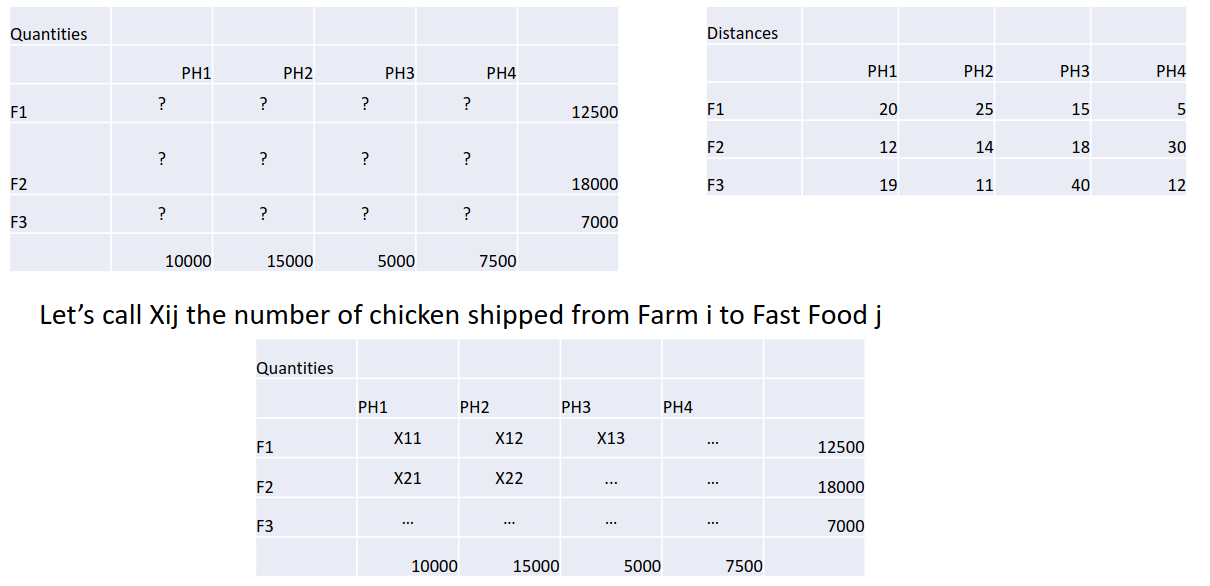
\includegraphics[width=0.95\textwidth]{./img/chichen-farm-variables.png}
  \end{center}
  \caption{}\label{fig:}
\end{figure}


Minimize and absolute value, we want to minimize the difference between the target and the value
\begin{align*}
  & \min{z} = |v - t| \\
  & \min{z} = |a| \\
  & |a| = \max{\{a, -a\}} \\
  & \min{z} = \max{\{a, -a\}} 
\end{align*}
we introduce an auxiliary variable $Y$
\begin{align*}
  & \min{z} = \min{Y} = \max{\{X_1, X_2\}} \\
  & Y >= X_1 \\
  & Y >= X_2 \\
  \\
  & \min{Y} \\
  & Y >= a \\
  & Y >= -a
\end{align*}

Example: 
...
We can express binary variables, $if X_1 > 0 then X_2 = 0$ and $if X_2 > 0 then X_1 = 0$. We can express them with binary variable $Y_1 = 0, 1$ $Y_2 = 0, 1$

BIG M, where M is constant, big fixed number. We want to express
\begin{align*}
  & Y_1 = 0, 1 \\
  & Y_2 = 0, 1 \\ 
  & Y_1 + Y_2 <= 1 \\ 
  & X_1 <= M_1 Y_1 \\ 
  & X_2 <= M_2 Y_2 
\end{align*}
If $Y_1$ is 0 $X_1$ is bount to 0, if $Y_1 = 1$ $X_1$ is virtually unbounded, the same for $X_2$ and $Y_2$. $M_1$ and $M_2$ are large constants. During a software simulation it reasonable to choose the varaibles in a range that won't be reachable.


\subsection{Fixed Values}
Problems where we have only a fixed amount of resources. We manage them by using several logical variable for every variable that is fixed.
\begin{align*}
  Y_1 + \dots + Y_k = 1 \\
  X = p_1 Y_1 + \dots + p_k Y_k
\end{align*}
The first equation imposes that only of the $Y$ can be one. The second equation imposes that $X_j$ can only have one of the quantities $p1, p2, \dots, p_k$.


Example 6:


A1, ..., A5
B1, ..., B5
C1, ..., C5
D1, ..., D5
we remove the years we cannot invest in.

we derive the first constraints starting from the first year. Wich is the sum of investments less than the total money.





\end{document}

%% vim: ts=2 sts=2 sw=2 et
